\chapter{Vaja: kadrovska}
\label{hw:klasifikacija}

Sedaj boste sami gradili modele in z njimi napovedovali. V gradniku File z namizja naložite podatke \textit{attrition-train.tab}.

\begin{marginfigure}
    \centering
    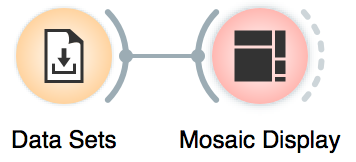
\includegraphics[width=50mm]{workflow1.png}
    \caption{$\;$}
    \label{fig:workflow1}
\end{marginfigure}

\hspace{1cm}

1) Z Mosaic Display najdite najlepšo projekcijo za dve spremenljivki? Kaj vam ta projekcija pove? Kakšen kader bo najhitreje odšel?

\begin{wrapfigure}{o}{1.0\textwidth}
    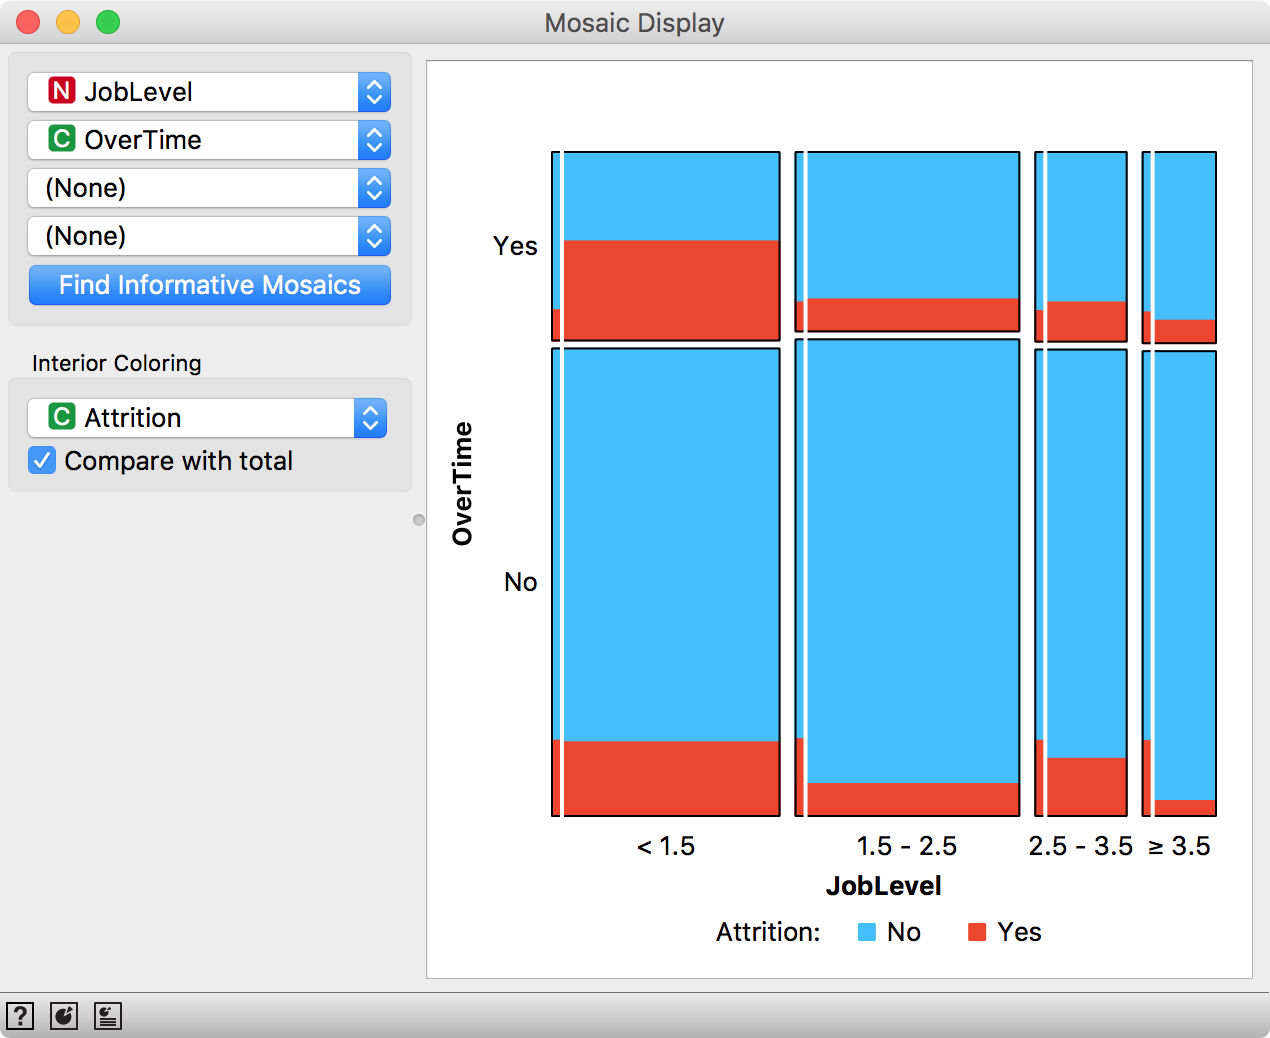
\includegraphics[scale=0.45]{mosaic.png}
    \caption{$\;$}
\end{wrapfigure}

2) Uporabite vse znane metode za napovedovanje in jih povežite v Test and Score. Katera metoda ima najvišjo klasifikacijsko točnost?

3) Katere tri spremenljivke so najpomembnejše za logistično regresijo? (Pozor! Target class morate nastaviti na ‘yes’.) Bi lahko razložili model? Kateri zaposleni bodo bolj verjetno dali odpoved?

\hspace{1cm}

Sedaj so nam iz kadrovske dostavili podatke za tri nove uslužbence. Kadrovsko službo zanima, kakšna je verjetnost, da bodo ti uslužbenci dali odpoved (za vsakega uslužbenca posebej). Uporabite podatke \textit{attrition-predict.tab}, jih naložite v File in napovejte verjetnosti z logistično regresijo.

4) Kdo od treh uslužbencev je najmanj zadovoljen (oz. bo verjetno dal odpoved)?

\begin{wrapfigure}{o}{1.0\textwidth}
    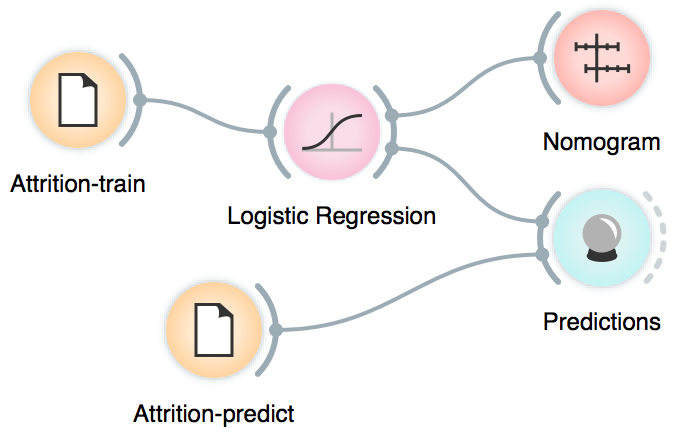
\includegraphics[scale=0.7]{workflow2.png}
    \caption{$\;$}
\end{wrapfigure}

5) Kaj mora kadrovska storiti, da bo uslužbenca zadržala? Namig: poglejte v Nomogram, zakaj uslužbenci odhajajo in povejte, s čim jih lahko prepričate, da ostanejo.